\documentclass[border=10pt]{standalone}
\usepackage{tikz}
\usetikzlibrary{calc, through}
\begin{document}
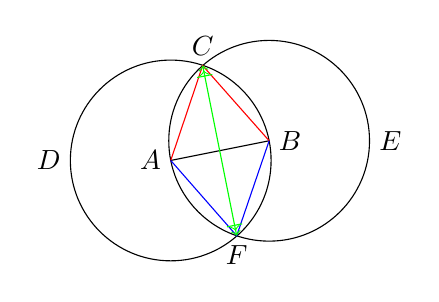
\begin{tikzpicture}
    \coordinate[label=left:{$A$}] (A) at (0, 0);
    \coordinate[label=right:{$B$}] (B) at (1.25, 0.25);
    \path[draw] (A) -- (B);
    \node (D) [draw, circle through = (B), label=left:{$D$}] at (A) {};
    \node (E) [draw, circle through = (A), label=right:{$E$}] at (B) {};
    \coordinate[label=above:{$C$}] (C) at (intersection 2 of D and E);
    \coordinate[label=below:{$F$}] (F) at 
    (intersection 1 of D and E);
    \path[draw, red] (A) -- (C) -- (B);
    \path[draw, blue] (A) -- (F) -- (B);
    \path[draw, <<|-|>>, green] (C) -- (F);

\end{tikzpicture}
\end{document}